%
% codage SAT-OPEN
%
\subsection{Nouveau codage SAT dans les espaces de plans}

\fred{A ajouter: complexité en espace meilleure par rapport à MK99}

Les codages SAT dans les espaces de plans existants introduits par \cite{DBLP:conf/aaai/MaliK99} se réfèrent tous à trois étapes indexées (pas nécessairement consécutives) du plan.
Dans notre nouveau codage, nous allons nous référer seulement à deux étapes consécutives.
Pour chaque action $\a\in\A$ et chaque étape $i$, nous créons une variable propositionnelle $\a_{i}$ pour déterminer qu'une instance de $\a$ doit être planifiée à l'étape $i$.
Pour chaque fluent $\f\in\F$ et chaque étape $i$, nous créons une variable propositionnelle $\open{\f}{i}$ pour exprimer que $\f$ se maintient à l'étape précédente $i-1$ et doit être protégé au moins jusqu'à l'étape $i$.

\begin{figure}[hb!]\centering
	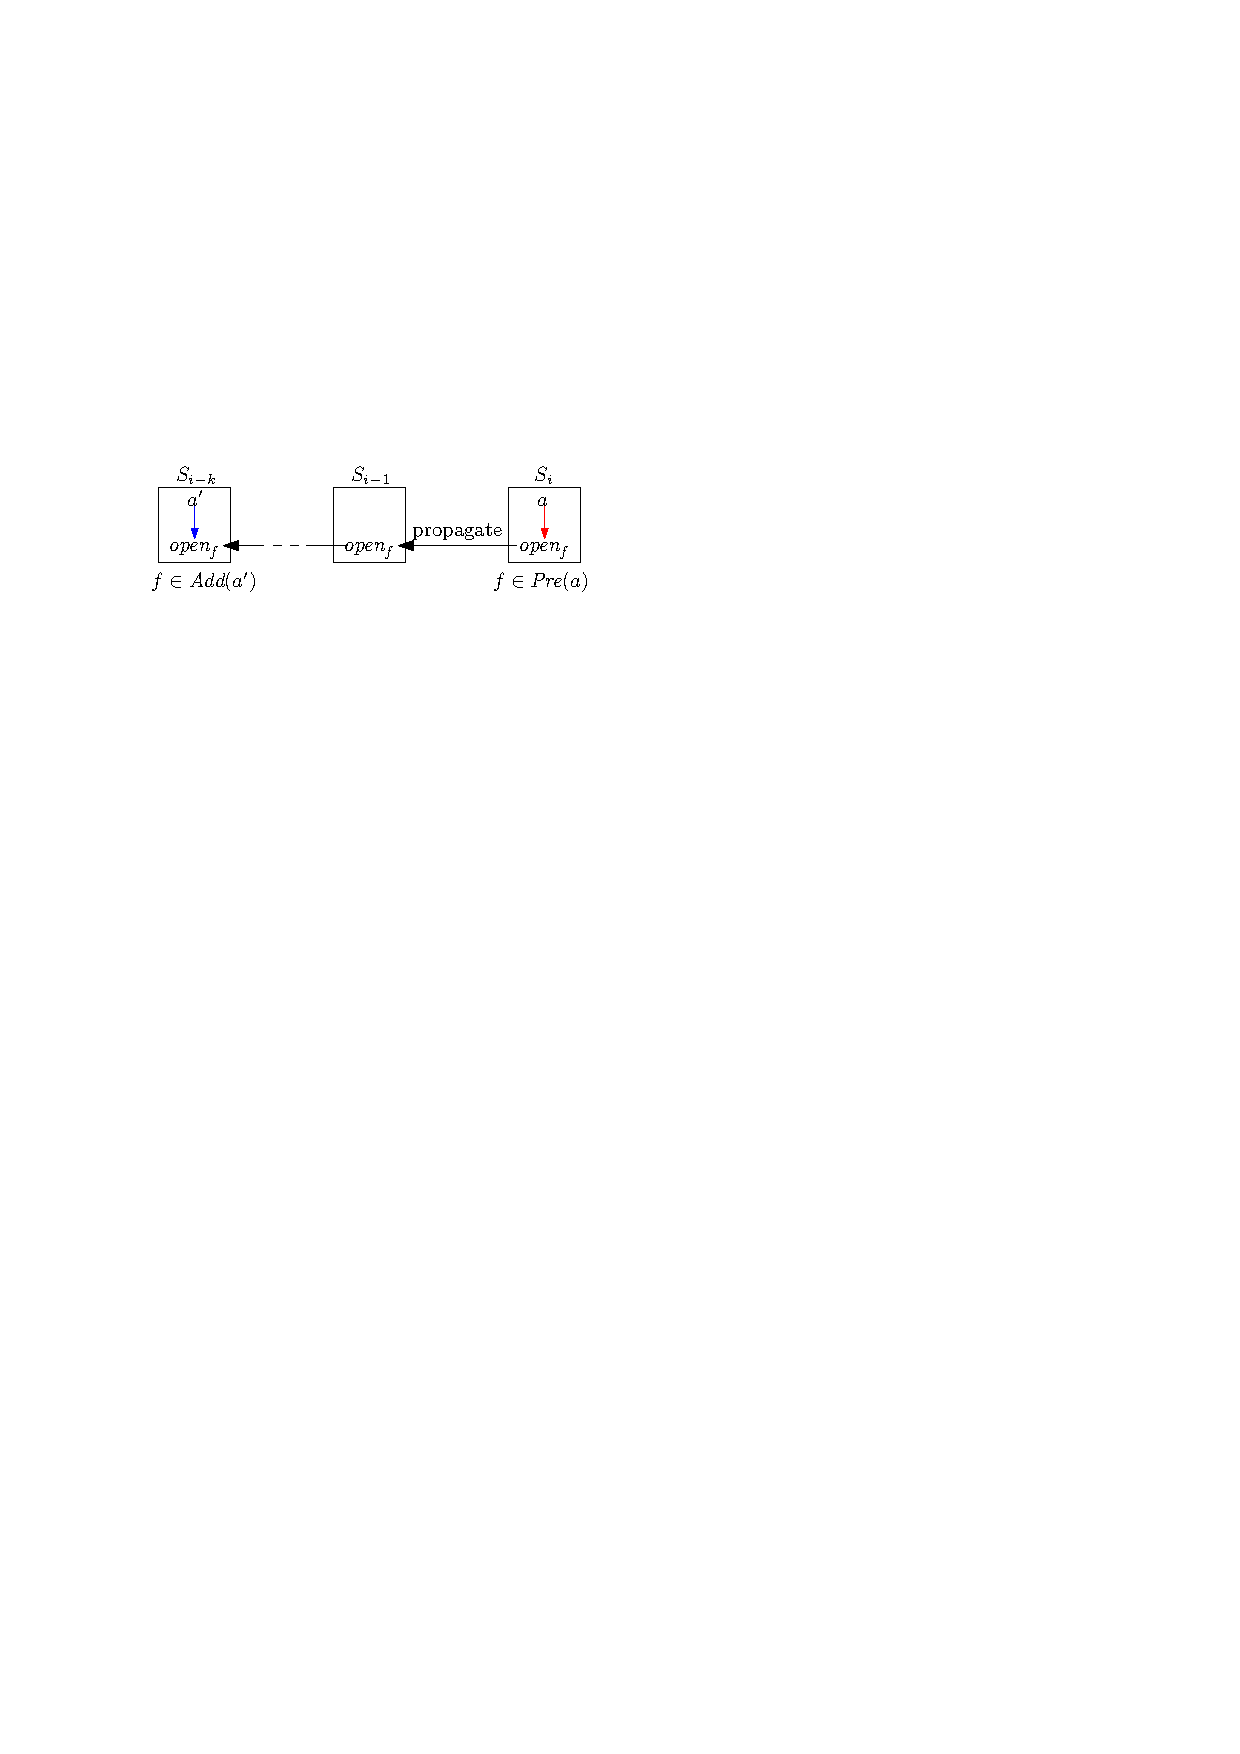
\includegraphics[width=.4\textwidth]{figures/transitions}
    \caption{Lien causal: l'action $a'$ produit $\f$ à l'étape $S_{i-k}$ pour l'action $\a$ qui nécessite $\f$ à l'étape $S_{i}$.}
    \label{fig:causal-link-sat}
\end{figure}

Dans la figure~\ref{fig:causal-link-sat}, la variable $f$ est une \textit {condition ouverte} à l'étape $\S_i$, impliquant que $\f\in\I$ ou une action $a'$ qui ajoute $\f$ est exécutée dans une étape précédente $\S_{i-k}$.
Les conditions ouvertes doivent être propagées vers l'arrière jusqu'à l'état initial ou une étape dans laquelle elles sont ajoutées par une action.




%\paragraph*{SAT Encodings for Classical Planning}
%%\begin{figure}\label{steps:sat}
%%\begin{tiny}
%%%(a)\\[1em]
%%  \xymatrix@C=0.1pc@R=1pc{
%%  \text{S}_{0} (\textit{Init}) \ar@{>}[r] & \fbox{$x_{1}\equiv$ S$_{1}$} \ar@{>}[r]  & \fbox{$x_{2}\equiv$ S$_{2}$} \ar@{>}[r] & \fbox{$x_{3}\equiv$ S$_{3}$} \ar@{>}[r] & \fbox{$x_{4}\equiv$ S$_{4}$}
%%  \ar@{>}[r] & \fbox{$x_{5}\equiv$ S$_{5}$} \ar@{>}[r] & \fbox{$x_{6}\equiv$ S$_{6}$} \ar@{>}[r] & \fbox{$x_{7}\equiv$ S$_{7}$} \ar@{>}[r] & \text{S}_{8} (\textit{Goal}) \\
%%  }
%%\end{tiny}
%%%(b)\\[1em]
%%%   \hspace{0.8em}\xymatrix@C=0pc@R=1pc{
%%%   & & & & & \fbox{$x_{2}\equiv$ S$_{4}$} \ar@{.}[lld] \ar@{.}[rrd] \ar@/^1pc/[rdd] & & & & \\
%%%   & & & \fbox{$x_{1}\equiv$ S$_{2}$} \ar[rd] & & & & \fbox{$x_{1}\equiv$ S$_{6}$} \ar[rd] & & \\
%%%   \text{S}_{0} (\textit{Init}) \ar@{>}[rr] & & \fbox{$x_{0}\equiv$ S$_{1}$} \ar[ru]  & & \fbox{$x_{0}\equiv$ S$_{3}$} \ar@/^1pc/[ruu] & &  \fbox{$x_{0}\equiv$ S$_{5}$} \ar[ru] & & \fbox{$x_{0}\equiv$ S$_{7}$} \ar@{>}[rr] & & \text{S}_{8} (\textit{Goal}) \\
%%%  }
%%\vspace{1em}
%%\caption{Transitions of an 8-steps plan in SAT/SMT encoding}
%%\end{figure}
%  Each step $i$ is associated with:\hfill
%  \begin{itemize}
%    \item a set of propositional variables for actions $\{a_{i}^{1},a_{i}^{2}\ldots,a_{i}^{m}\}$
%    \item a set of propositional variables for open conditions $\{open_{f^1,i},open_{f^2,i},\ldots,open_{f^n,i}\}$ %which determine their value in state $x_{i-1}$
%  \end{itemize}


%\begin{frame}{SAT Encoding: open conditions}
%Given a propositional formula $\varphi$, $\textit{open}_{\varphi} = \textit{NNF}_{\textit{open}}(+1,\varphi)$ with:\\[0.8em]
%\begin{itemize}
%  \item $\textit{NNF}_{\textit{open}}(+1,f) = \textit{open}_{f}$
%  \item $\textit{NNF}_{\textit{open}}(-1,f) = \textit{open}_{\neg f}$\\[0.8em]
%  \item $\textit{NNF}_{\textit{open}}(+1,\neg \varphi) = \textit{NNF}_{\textit{open}}(-1,\varphi)$
%  \item $\textit{NNF}_{\textit{open}}(-1,\neg \varphi) = \textit{NNF}_{\textit{open}}(+1,\varphi)$\\[0.8em]
%  \item $\textit{NNF}_{\textit{open}}(+1,\varphi_{1} \wedge \varphi_{2}) = \textit{NNF}_{\textit{open}}(+1,\varphi_{1}) \wedge \textit{NNF}_{\textit{open}}(+1,\varphi_{2})$
%  \item $\textit{NNF}_{\textit{open}}(-1,\varphi_{1} \wedge \varphi_{2}) = \textit{NNF}_{\textit{open}}(-1,\varphi_{1}) \vee \textit{NNF}_{\textit{open}}(-1,\varphi_{2})$\\[0.8em]
%   \item $\textit{NNF}_{\textit{open}}(+1,\varphi_{1} \vee \varphi_{2}) = \textit{NNF}_{\textit{open}}(+1,\varphi_{1}) \vee \textit{NNF}_{\textit{open}}(+1,\varphi_{2})$
%   \item $\textit{NNF}_{\textit{open}}(-1,\varphi_{1} \vee \varphi_{2}) = \textit{NNF}_{\textit{open}}(-1,\varphi_{1}) \wedge \textit{NNF}_{\textit{open}}(-1,\varphi_{2})$\\[0.8em]
%\end{itemize}
%\end{frame}


%\paragraph*{SAT Encoding: open conditions, then propagate or close}

Dans la suite, nous donnons notre codage pour une longueur de plan fixée $\length$. Une borne supérieure pour $\length$ est le nombre total d'états possibles, soit $2^{\mid\F\mid}$.

\paragraph*{Conditions ouvertes}

Si une action $\a$ est exécutée dans une étape du plan, alors chaque condition de $\a$ doit être une condition ouverte à cette étape (c'est-à-dire qu'un lien causal est requis pour cette condition).


\begin{small}
\begin{multline*}
~\\[-3em]
\bigwedge\limits_{\substack{\mathbf{i}\in [1..\mathbf{\length}]}}\bigwedge\limits_{\substack{\mathbf{\a}\in \mathbf{\A}}}\left(\mathbf{\a}_{\mathbf{i}} \Rightarrow \bigwedge\limits_{\substack{\mathbf{\f}\in \pre{\mathbf{\a}}}}open_{\mathbf{\f},\mathbf{i}}\right)\hfill\\[-2em]
%%%
\end{multline*}
\end{small}

Dans la dernière étape du plan menant au but tous les fluents du but doivent être des conditions ouvertes ou ajoutées par des actions exécutées dans cette étape.

\begin{small}
\begin{multline*}
~\\[-3em]
\bigwedge\limits_{\substack{\mathbf{\f}\in \mathbf{\G}}}\left(open_{\mathbf{\f},\mathbf{\length}} \vee \bigvee\limits_{\substack{\mathbf{\a}\in \mathbf{\A}\\\mathbf{\f} \in \add{\mathbf{\a}}}}\mathbf{\a}_{\mathbf{\length}}\right)\hfill\\[-2em]
%%%
\end{multline*}
\end{small}

\paragraph*{Propagation et fermeture}

Aucune condition ne doit rester ouverte dans la première étape du plan si elle n'est pas fournie dans l'état initial.
%$\bigwedge_{\mathbf{\f}\in \mathbf{\F}\setminus \mathbf{I}}\neg open_{\mathbf{\f},1}$

\begin{small}
\begin{multline*}
~\\[-3em]
\bigwedge\limits_{\substack{\mathbf{\f}\in \mathbf{\F}\setminus \mathbf{I}}}\neg open_{\mathbf{\f},1}\hfill\\[-2em]
%%%
\end{multline*}
\end{small}

Toute condition ouverte dans une étape doit soit rester ouverte soit être ajoutée (fermée) par une action à l'étape précédente.

\begin{small}
\begin{multline*}
~\\[-3em]
\bigwedge\limits_{\substack{\mathbf{i}\in [2..\mathbf{\length}]}}\bigwedge\limits_{\substack{\mathbf{f}\in \mathbf{\F}}}\left(open_{\mathbf{\f},\mathbf{i}} \Rightarrow \left(open_{\mathbf{\f},\mathbf{i} - 1} \vee \bigvee\limits_{\substack{\mathbf{\a}\in \mathbf{\A}\\\mathbf{\f} \in \add{\mathbf{\a}}}}\mathbf{\a}_{\mathbf{i} - 1}\right)\right)\hfill\\[-2em]
%%%
\end{multline*}
\end{small}


%\paragraph*{SAT Encoding: protect open conditions and prevent negative interactions (mutex)}

\paragraph*{Protection des conditions ouvertes}

Une condition ouverte dans une étape donnée ne peut pas être supprimée à l'étape précédente. Cela garantit de ne rompre aucun lien de causalité dans le plan.
\begin{small}
\begin{multline*}
~\\[-3em]
\bigwedge\limits_{\substack{\mathbf{i}\in [2..\mathbf{\length}]}}\bigwedge\limits_{\substack{\mathbf{\f}\in \mathbf{\F}}}\left(open_{\mathbf{\f},\mathbf{i}} \Rightarrow \bigwedge\limits_{\substack{\mathbf{\a}\in \mathbf{\A}\\\mathbf{\f} \in \del{\mathbf{\a}}}}\neg \mathbf{\a}_{\mathbf{i} - 1}\right)\hfill\\[-3em]
%%%
\end{multline*}
\end{small}

\paragraph*{Prévention des interactions négatives}

Si une action supprime un fluent qui est nécessaire ou est ajouté par une autre action, alors ces deux actions ne peuvent pas être exécutées toutes les deux dans une même étape.

\begin{small}
\begin{multline*}
~\\[-3em]
\bigwedge\limits_{\substack{\mathbf{i}\in [1..\mathbf{length}]}}\bigwedge\limits_{\substack{\mathbf{\a}\in \mathbf{\A}}}\bigwedge\limits_{\substack{\mathbf{f}\in \left(\add{\mathbf{\a}}\cup\pre{\mathbf{\a}}\right)}}\bigwedge\limits_{\substack{\mathbf{\b}\in \mathbf{\A}\\\mathbf{\a} \neq \mathbf{\b} \wedge \mathbf{f} \in \del{\mathbf{\b}}}}\left(\neg \mathbf{\a}_{\mathbf{i}} \vee \neg \mathbf{\b}_{\mathbf{i}}\right)\hfill\\[-3em]
\end{multline*}
\end{small}


Dans la section suivante, nous présentons une version plus compacte de ce nouveau codage qui utilise le langage QBF. Nous étendons ensuite ce codage SAT pour la planification classique en un codage SMT pour la planification temporelle en temps continu.
